\documentclass[11pt,twocolumn,oneside,openany,headings=optiontotoc,11pt,numbers=noenddot]{article}

\usepackage[a4paper]{geometry}
\usepackage[utf8]{inputenc}
\usepackage[T1]{fontenc}
\usepackage{lmodern}
\usepackage[ngerman]{babel}
\usepackage{ngerman}

\usepackage[onehalfspacing]{setspace}

\usepackage{fancyhdr}
\usepackage{fancybox}

\usepackage{rotating}
\usepackage{varwidth}

%Struktogramme
\usepackage[german,curves]{struktex}

\usepackage{pdflscape}
\usepackage{changepage}
\usepackage{graphicx}
\usepackage[bottom]{footmisc}
\usepackage{transparent}
\usepackage{graphbox}
\graphicspath{
	{Pics/PDFs/}
	{Pics/JPGs/}
	{Pics/PNGs/}
}
\usepackage{caption}
\usepackage{wrapfig}
\usepackage{marginnote}
\usepackage{tabularx}
\usepackage{dashrule}
\usepackage{soulutf8}
\usepackage{hhline}
%arydshln suppresses vertical lines in table
%\usepackage{arydshln}
\usepackage{multirow}
\usepackage{enumerate}
\usepackage[hidelinks]{hyperref}
\usepackage{listings}

\usepackage[table]{xcolor}
\usepackage{array}
\usepackage{enumitem,amssymb,amsmath}
\usepackage{interval}
\usepackage{cancel}
\usepackage{stmaryrd}
\usepackage{wasysym}
\usepackage{polynom}
\usepackage{diagbox}
\usepackage{dashrule}
\usepackage{framed}
\usepackage{mdframed}
\usepackage{karnaugh-map}
\usepackage{pdfpages}

\usepackage{blindtext}

\usepackage{eso-pic}

\usepackage{amssymb}
\usepackage{eurosym}

\usepackage[pages=some]{background}
\pagestyle{headings}
\renewcommand{\headrulewidth}{0.2pt}
\renewcommand{\footrulewidth}{0.2pt}
\newcommand*{\underdownarrow}[2]{\ensuremath{\underset{\overset{\Big\downarrow}{#2}}{#1}}}
\setlength{\fboxsep}{5pt}
\newcommand{\explainBelow}[3]{\underbrace{#1}_{\parbox{\widthof{#3}}{\footnotesize\raggedright #2}}}
\newcommand{\explainAbove}[3]{\overbrace{#1}^{\parbox{\widthof{#3}}{\footnotesize\raggedright #2}}}
\newcommand\footnoteref[1]{\protected@xdef\@thefnmark{\ref{#1}}\@footnotemark}


% Codestyle defined
\definecolor{codegreen}{rgb}{0,0.6,0}
\definecolor{codegray}{rgb}{0.5,0.5,0.5}
\definecolor{codepurple}{rgb}{0.58,0,0.82}
\definecolor{backcolour}{rgb}{0.95,0.95,0.92}
\definecolor{deepgreen}{rgb}{0,0.5,0}
\definecolor{darkblue}{rgb}{0,0,0.65}
\definecolor{mauve}{rgb}{0.40, 0.19,0.28}
\colorlet{exceptioncolour}{yellow!50!red}
\colorlet{commandcolour}{blue!60!black}
\colorlet{numpycolour}{blue!60!green}
\colorlet{specmethodcolour}{violet}

%Neue Spaltendefinition
\newcolumntype{L}[1]{>{\raggedright\let\newline\\\arraybackslash\hspace{0pt}}m{#1}}
\newcolumntype{M}{>{\centering\arraybackslash}X}
\newcommand{\cmnt}[1]{\ignorespaces}
%Textausrichtung ändern
\newcommand\tabrotate[1]{\rotatebox{90}{\raggedright#1\hspace{\tabcolsep}}}

%Intervall-Konfig
\intervalconfig {
	soft open fences
}

%Bash
\lstdefinestyle{BashInputStyle}{
	language=bash,
	basicstyle=\small\sffamily,
	backgroundcolor=\color{backcolour},
	columns=fullflexible,
	backgroundcolor=\color{backcolour},
	breaklines=true,
}
%Java
\lstdefinestyle{JavaInputStyle}{
	language=Java,
	backgroundcolor=\color{backcolour},
	aboveskip=1mm,
	belowskip=1mm,
	showstringspaces=false,
	columns=flexible,
	basicstyle={\footnotesize\ttfamily},
	numberstyle={\tiny},
	numbers=none,
	keywordstyle=\color{purple},,
	commentstyle=\color{deepgreen},
	stringstyle=\color{blue},
	emph={out},
	emphstyle=\color{darkblue},
	emph={[2]rand},
	emphstyle=[2]\color{specmethodcolour},
	breaklines=true,
	breakatwhitespace=true,
	tabsize=2,
}
%Python
\lstdefinestyle{PythonInputStyle}{
	language=Python,
	alsoletter={1234567890},
	aboveskip=1ex,
	basicstyle=\footnotesize,
	breaklines=true,
	breakatwhitespace= true,
	backgroundcolor=\color{backcolour},
	commentstyle=\color{red},
	otherkeywords={\ , \}, \{, \&,\|},
	emph={and,break,class,continue,def,yield,del,elif,else,%
		except,exec,finally,for,from,global,if,import,in,%
		lambda,not,or,pass,print,raise,return,try,while,assert},
	emphstyle=\color{exceptioncolour},
	emph={[2]True,False,None,min},
	emphstyle=[2]\color{specmethodcolour},
	emph={[3]object,type,isinstance,copy,deepcopy,zip,enumerate,reversed,list,len,dict,tuple,xrange,append,execfile,real,imag,reduce,str,repr},
	emphstyle=[3]\color{commandcolour},
	emph={[4]ode, fsolve, sqrt, exp, sin, cos, arccos, pi,  array, norm, solve, dot, arange, , isscalar, max, sum, flatten, shape, reshape, find, any, all, abs, plot, linspace, legend, quad, polyval,polyfit, hstack, concatenate,vstack,column_stack,empty,zeros,ones,rand,vander,grid,pcolor,eig,eigs,eigvals,svd,qr,tan,det,logspace,roll,mean,cumsum,cumprod,diff,vectorize,lstsq,cla,eye,xlabel,ylabel,squeeze},
	emphstyle=[4]\color{numpycolour},
	emph={[5]__init__,__add__,__mul__,__div__,__sub__,__call__,__getitem__,__setitem__,__eq__,__ne__,__nonzero__,__rmul__,__radd__,__repr__,__str__,__get__,__truediv__,__pow__,__name__,__future__,__all__},
	emphstyle=[5]\color{specmethodcolour},
	emph={[6]assert,range,yield},
	emphstyle=[6]\color{specmethodcolour}\bfseries,
	emph={[7]Exception,NameError,IndexError,SyntaxError,TypeError,ValueError,OverflowError,ZeroDivisionError,KeyboardInterrupt},
	emphstyle=[7]\color{specmethodcolour}\bfseries,
	emph={[8]taster,send,sendMail,capture,check,noMsg,go,move,switch,humTem,ventilate,buzz},
	emphstyle=[8]\color{blue},
	keywordstyle=\color{blue}\bfseries,
	rulecolor=\color{black!40},
	showstringspaces=false,
	stringstyle=\color{deepgreen}
}

\lstset{literate=%
	{Ö}{{\"O}}1
	{Ä}{{\"A}}1
	{Ü}{{\"U}}1
	{ß}{{\ss}}1
	{ü}{{\"u}}1
	{ä}{{\"a}}1
	{ö}{{\"o}}1
}

% Neue Klassenarbeits-Umgebung
\newenvironment{worksheet}[3]
% Begin-Bereich
{
	\newpage
	\sffamily
	\setcounter{page}{1}
	\ClearShipoutPicture
	\AddToShipoutPicture{
		\put(55,761){{
				\mbox{\parbox{385\unitlength}{\tiny \color{codegray}BBS I Mainz, #1 \newline #2
						\newline #3
					}
				}
			}
		}
		\put(455,761){{
				\mbox{\hspace{0.3cm}
\includegraphics[width=0.2\textwidth]{../../logo.pdf}}
			}
		}
	}
}
% End-Bereich
{
	\clearpage
	\ClearShipoutPicture
}

\setlength{\columnsep}{3em}
\setlength{\columnseprule}{0.5pt}

\geometry{left=2.00cm,right=2.00cm,top=3.00cm,bottom=1.00cm,includeheadfoot}
\pagenumbering{gobble}
\pagestyle{empty}

\begin{document}
	\begin{worksheet}{BS FI 16}{2. Lehrjahr, LF 9 - Öffentliche Netze}{Informationen zur Auswahl der Access Point}
		\section{Auswahl der Access Point}
		Bei der Planung einer Netzwerkerweiterung um WLAN spielt die verwendete Hardware natürlich eine zentrale Rolle. Das bedeutet, die Qualität der Signalabdeckung kann maßgeblich beeinflusst werden von den verwendeten Access Points (AP).\\
		Ein grundlegender Unterschied ist der vom AP verwendete Frequenzbereich. Dabei sind zwei Frequenzbereiche zu unterscheiden:
		\begin{itemize}
			\item 2,4GHz: bietet eine bessere Reichweite im Vergleich zum 5GHz-Bereich; Überlappung mit benachbarten AP wahrscheinlicher $\Rightarrow$ 3/10 Kanälen überlappungsfrei nutzbar
			\item 5GHz: starke Begrenzung durch Wände und andere Hindernisse; höhere nutzbare Kanalanzahl
		\end{itemize}
		Nun folgt durch den gewählten Frequenzbereich eine Einschränkung auf bestimmte Funkstandards.
		\begin{itemize}
			\item 2,4GHz: \textit{802.11, 802.11b, 802.11g} und \textit{802.11n}
			\item 5GHz: \textit{802.11a/h, 802.11ac} und \textit{802.11n}
		\end{itemize}
		Während die Standards 802.11b und 802.11g lediglich das Senden über \underline{eine} Antenne anbieten, kann mit 802.11n eine parallele Datenübertragung au mehreren Kanälen ermöglicht werden.\\
		Zusätzlich zu den möglichen Frequenzbereichen, den daraus resultierenden Standards und Übertragungsraten können die nachfolgend aufgelisteten Aspekte einen Einfluss auf die Entscheidung haben:
		\begin{itemize}
			\item Power over Ethernet (PoE) Fähigkeit des AP: ermöglicht eigenständiges Betreiben ohne externe Energieversorgung
			\item Simultane Funknetz-ID Unterstützung (SSID)
			\item komplette IP-Bereichabdeckung
			\item Unterstützung dynamische IP-Konfiguration (DHCP)
			\item zentrale Verwaltung möglich
			\item WPA2-Enterprise-fähig
			\item[] Abhängig vom Einsatzbereich kann sollte auch noch berücksichtigt werden, ob
			\item Seamless-Roaming-fähig
			\item aktive Lastverteilung
		\end{itemize}
		Abhängig von der gewählten Frequenz kann ein AP \(10-30\) Meter abdecken.\\
		Bei 2,4GHz ist der Abdeckungsbereich größer, aber auch hier ist das Signal an den Rändern schwach. Bei 5GHz kann eine ähnlich große Fläche abgedeckt werden, wobei hier die Signalstärke bereits früher abnimmt.\\
		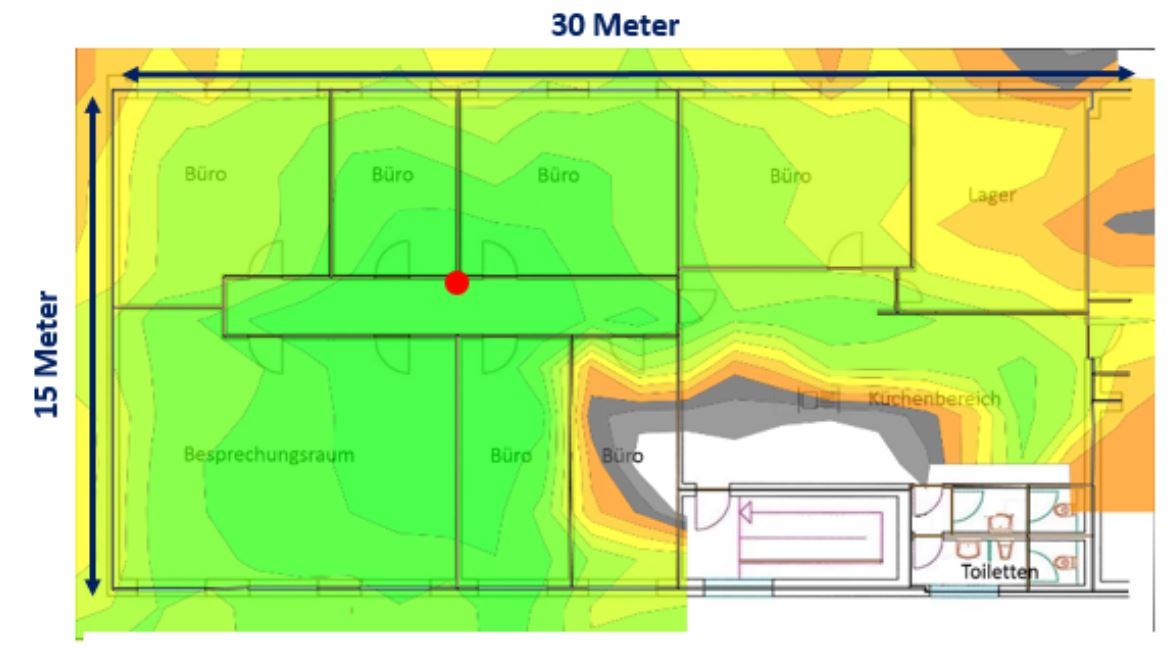
\includegraphics[scale=0.4]{Bilder/2,4ghz.jpg}\\
		\tiny{Frequenzbereich: 2,4GHz - Trockenbauwände - \href{https://www.enbitcon.de/shop/sophos-ap-55-access-point?gclid=EAIaIQobChMI05evyPyx2wIVGp7VCh1IHgJSEAQYAiABEgKC6fD_BwE07}{enbitcon.com}}\normalsize\\
		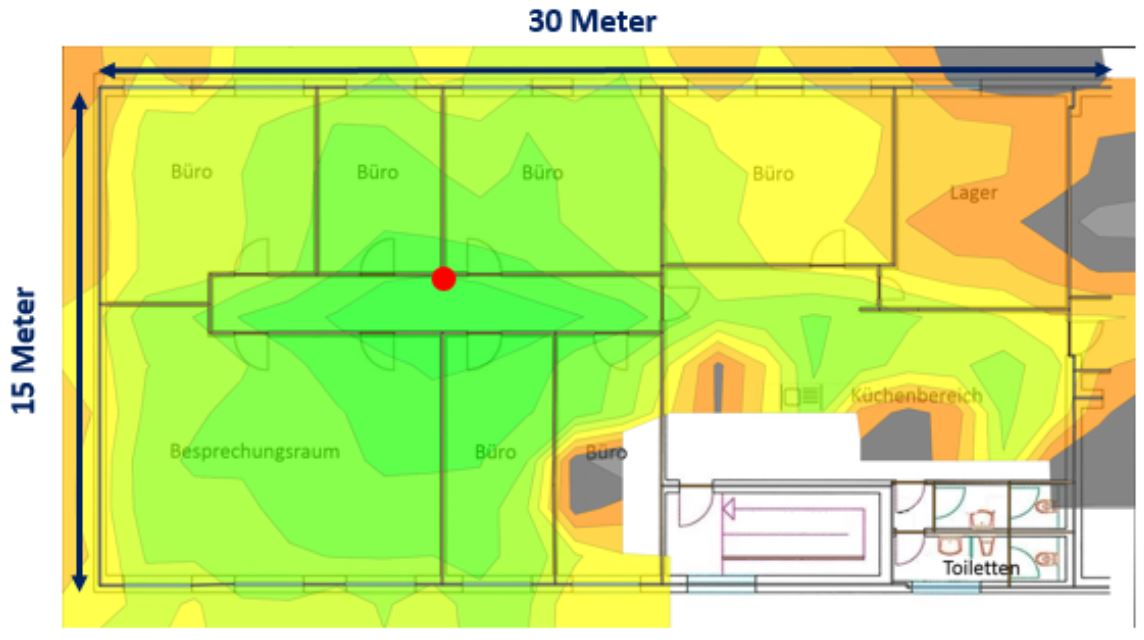
\includegraphics[scale=0.4]{Bilder/5ghz.jpg}
		\tiny{Frequenzbereich: 5GHz - Trockenbauwände - \href{https://www.enbitcon.de/shop/sophos-ap-55-access-point?gclid=EAIaIQobChMI05evyPyx2wIVGp7VCh1IHgJSEAQYAiABEgKC6fD_BwE07}{enbitcon.com}5}\normalsize\\
		Mit der Wahl der Frequenz ist es aber noch nicht getan. Ebenfalls muss entschieden werden, auf welchem Kanal der AP funkt. Um Signalüberdeckungen zu vermeiden, sollten für die entsprechenden Frequenzen nur um jeweils drei versetzte Kanäle verwendet werden!\\
		\par\noindent
		\begin{tabularx}{0.5\textwidth}{X|X}
			2,4GHz & 5GHz\\
			\hline
			1 & 52\\
			5 & 56\\
			9 & 60\\
			13 & 64\\
			& 100\\
			& 104\\
			& 108\\
			& 112\\
			& 136\\
			& 140\\
			\cline{2-2}\\
			& nur mit Einschränkung\\
			\cline{2-2}
			& 36 - Indoor!\\
			& 40 - Indoor!\\
			& 44 - Indoor!\\
			& 48 - Indoor!\\
			& 116 - Radar!\\
			& 120 - Radar!\\
			& 124 - Radar!\\
			& 128 - Radar! (Wetterradar in Rostock/Warnemünde)\\
			& 132 - Radar!\\
		\end{tabularx}\\
		\tiny{\href{https://wiki.opennet-initiative.de/wiki/WLAN_Frequenzen#Nutzbare_WLAN_Kan.C3.A4le}{wiki.opennet-initiative.de}}\normalsize
		\newpage \noindent
		\section*{Antennen}
		Zusätzlich zu den internen Spezifikationen, die ein AP mit sich bringt, kann auch die Antennenausstattung des AP eine interessante Rolle in der Entscheidungsfindung spielen.\\
		Auch bei den Antennen gibt es Unterschiede, so dass auch hier der Einsatzbereich und die Anforderungen an das WLAN berücksichtigt werden müssen. Es lässt sich im groben zwischen
		\begin{itemize}
			\item \textit{omni-direktionaler Rundstrahl-Antenne}: sendet Funk ähnlich einer Glühbirne (Form eines dicken Donut). Das heißt, diese Antenne strahlt horizontal \(360^\circ\) in alle Richtungen, beschränkt sich vertikal aber nur auf das nötigste.\\
			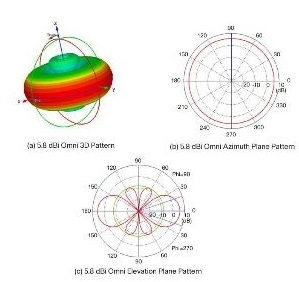
\includegraphics[scale=0.75]{Bilder/omni.png}\\
			\tiny{\href{https://www.computerwoche.de/g/wlan-antennen-und-access-points-richtig-positionieren,37573,5#galleryHeadline}{Computerwoche}}\normalsize
			\item \textit{Direktionaler Sektor-Antenne}: die Ausstrahlung lässt sich mit dem Lichtkegel einer Taschenlampe vergleichen, das Funkmuster ähnelt einer Birne oder einem Apfel mit identischem horizontalen und vertikalen Öffnungswinkel (\(60^\circ, 90^\circ\) oder \(120^\circ\)).\\
			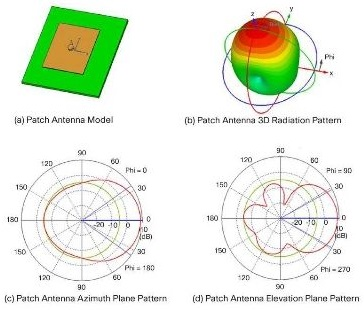
\includegraphics[scale=0.75]{Bilder/dirSek.jpg}\\
			\tiny{\href{https://www.computerwoche.de/g/wlan-antennen-und-access-points-richtig-positionieren,37573,8#galleryHeadline}{Computerwoche}}\normalsize
			\newpage
			\item \textit{Direktionaler Richt-Antenne}: bündelt die ausgesendeten Funkstrahlen in ein Richtung, das Funkmuster kann mit einer Salatgurke veglichen werden, wobei sich der Öffnungswinkel horizontal und vertikal um ca. \(6^\circ\) bewegt.
			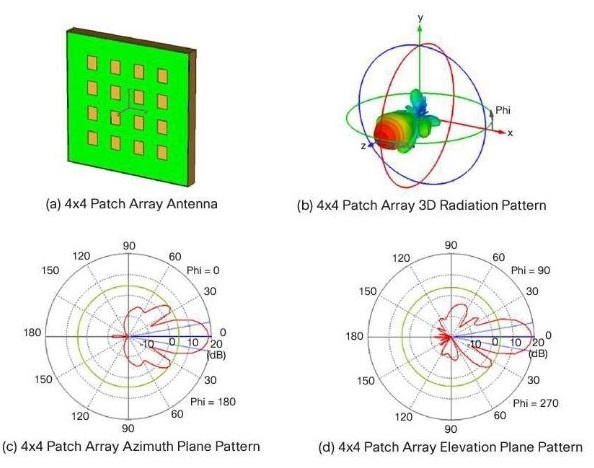
\includegraphics[scale=0.75]{Bilder/dirRich.jpg}\\
			\tiny{\href{https://www.computerwoche.de/g/wlan-antennen-und-access-points-richtig-positionieren,37573,4#galleryHeadline}{Computerwoche}}\normalsize
		\end{itemize}
		unterschieden werden.\\
		Möchte man größere Gebäudekomplexe mit einem WLAN versorgen, benötigt man eine entsprechend große Auswahl an Antennen. Eine externe Antenne ermöglicht einen größeren Gestaltungs- und Optimierungs-Spielraum als interne Antennen.
		\subsection*{Omnidirektionale Rundstrahl-Antennen} Diese Antennen werden häufig in der mitte des Raumes positioniert, so dass sie im optimalsten Falle alle im in der Nähe befindlichen Clients erreichen und mit Wireless-Funk versorgen. Genutzt werden diese Art von Antennen um funktechnisch unkomplizierte Räume (wenig Störquellen) zu versorgen.\\
		Bei einer solchen Rundstrahl-Antenne unterscheidet man zwischen Antennen mit einem und mit mehreren Dipol-Drähten. Der Unterschied ist hier in der horizontalen bzw. vertikalen Reichweite. Währen Antennen mit einem Dipol-Draht eine höhere vertikale aber geringere horizontale Ausstrahlung haben, decken Antennen mit mehreren Dipol-Drähte horizontal eine größere Fläche ab, können dafür aber vertikal nicht soweit ausstrahlen.
		\subsection*{Direktionale Sektor-Antenne} Eine solche Antenne sendet horizontal und vertikal in einem ähnlichen Winkel (\(60^\circ, 90^\circ\) oder \(120^\circ\)).\\
		Solche Antennen, genauer gesagt die \(120^\circ\) Antennen werden an Mobilfunkmasten verwendet und sorgen im Dreier-Gespann für eine \(360^\circ\) Abdeckung. Ähnlich zu diesem Prinzip können AP-Antennen ausgerichtet werden um eine \(360^\circ\) WLAN-Abdeckung zu gewährleisten. Diese Kombination aus einzelnen Sektor-Antennen ermöglicht die Abdeckung eines größeren Bereichs (Reichweite).
		\subsection*{Direktionale Richt-Antennen} Diese Form der Antennen können mit den Sektor-Antennen verglichen werden, wobei sie die Funkstrahlung stärker bündeln und somit eine noch größere Reichweite haben.\\
		Korrekt ausgerichtet kann diese Art von Antenne bis zu 20 km überbrücken.\\
		\hdashrule[0.5ex][x]{0.45\textwidth}{0.1mm}{8mm 2pt}\\
		An APs werden häufig zwei oder mehrere identische Antennen verwendet. Dieser Umstand ist durch eine gewünschte Reduzierung der Interferenzen bedingt (\textbf{Diversity-Antennen}).\\
		Da die angebrachten Antennen an APs ein wenig voneinander entfernt befinden, werden die Funksignale unterschiedlich von den umgebenden Oberflächen reflektiert und erreichen so den Client zu minimal unterschiedlichen Zeitpunkten und mit unterschiedlicher Qualität. Der Client wechselt nun immer auf die Antenne, die das bessere Signal sendet.\\
		\par\noindent
		APs die den Standard 802.11n bzw. 802.11ac unterstützen verwenden das sogenannte MIMO\footnote{Multiple-Input Multiple Output}-Multi-Connection-Multi-Antennen-Verfahren. Dieses Verfahren verwendet mehrere Antennen zum Senden und Empfangen von Daten.
		\par\bigskip\noindent
		\tiny{Quellen:\\
			- \href{https://lehrerfortbildung-bw.de/st_digital/tablet/anleitungen/infrastruktur/wlan/ap-auswahl.html}{Lehrerfortbildung} (eingesehen: 31.05.2018)\\
			- \href{https://www.computerwoche.de/a/wlan-ratgeber-antennen-richtig-waehlen-und-positionieren,3060831}{Computerwoche} (eingesehen: 31.05.2018)}
	\end{worksheet}
\end{document}